\chapter{Feedback Theory}
\label{ch:feedback}

When we talk about feedback, we mean that part of the output signal is fed back to the input. What is applied to the input of the circuit is not the input signal, but rather the difference between input signal and the returned output signal.

We will see in this chapter that feedback offers many advantages:
\begin{itemize}
	\item It allows for accurate gain control,
	\item You can control the input and output impedance,
	\item You can extend the bandwidth,
	\item The distortions are reduced
\end{itemize}
We discuss these topics in turn, and afterwards have a look at some stability issues that may arise by applying feedback.

\section{Accurate Gain Control}
In figure \ref{fig:feedback_general}, the output voltage $v_o$, generated by an amplifier with transmittance $A(j\omega)$,  is returned to the input through a system with transmittance $H(j\omega)$. We can write:
\begin{equation}
\begin{split}
	v_f &= H(j\omega) \; v_o \\
	v_c &= v_i - v_f = v_i - H(j\omega) \; v_o\\
	v_o &= A(j\omega) \; v_c  = A(j\omega) \; (v_i - H(j\omega) \; v_o) \\
	%\Rightarrow (1 + A(j\omega) \; H(j\omega)) \; v_o = A(j\omega) \; v_i  \\
	\Rightarrow A_{CL} = \frac{v_o}{v_i} &= \frac{A(j\omega)}{1 + A(j\omega) \; H(j\omega)} \\
										&= \frac{A}{1 + AH} = \frac{A}{1 + T}
\end{split}
\label{eq:closed-loop}
\end{equation}

\begin{minipage}{.5\textwidth}
	\centering
	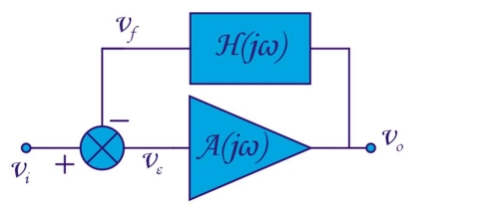
\includegraphics[width=9cm]{figures/ch10/feedback_general.jpg}
	\captionof{figure}{}
	\label{fig:feedback_general}
\end{minipage}%
\begin{minipage}{.5\textwidth}
	\centering
	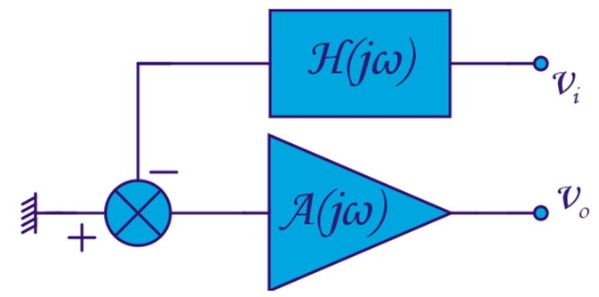
\includegraphics[width=7cm]{figures/ch10/feedback2.jpg}
	\captionof{figure}{}
	\label{fig:feedback}
\end{minipage}

Some definitions: $A$ is the open-loop gain and $H$ the feedback gain, $A_{CL}$ is called the  closed-loop gain and $T = AH$ is the \emph{loop gain}. The loop gain $T$ can be obtained by this procedure:
\begin{enumerate}
	\item Open the feedback loop at the amplifier output,
	\item Ground the input,
	\item Apply $v_i$ at the open end of the loop,
	\item Obtain $T$ by computing $v_o/v_i$.
\end{enumerate}
This method is visualized in figure \ref{fig:feedback}, where we applied it to the circuit in \ref{fig:feedback_general}. The signal at the input of the amplifier is $H\;v_i$, and $v_o = A H \; v_i$, so we find the loop gain.

\begin{minipage}{.5\textwidth}
	\centering
	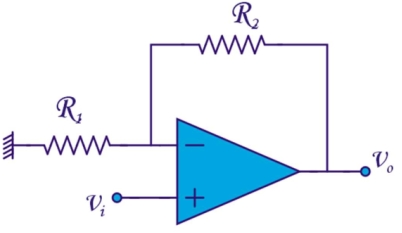
\includegraphics[width=7cm]{figures/ch02/opamp4.jpg}
	\captionof{figure}{}
	\label{fig:feedback2}
\end{minipage}%
\begin{minipage}{.5\textwidth}
	\centering
	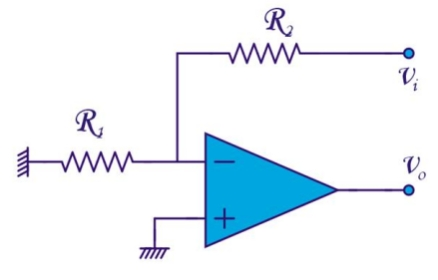
\includegraphics[width=7cm]{figures/ch10/feedback3.jpg}
	\captionof{figure}{}
	\label{fig:feedback3}
\end{minipage}

When we apply this to the non-inverting OPAMP topology that we saw in section \ref{sec:opamp}, which is pictured in \ref{fig:feedback2}, we get the circuit in figure \ref{fig:feedback3} with the feedback loop opened and the input grounded. The voltage at the negative terminal is $v^- = \frac{R_1}{R_1 + R_2} v_i$, and the output is then $v_o = -A\;\frac{R_1}{R_1 + R_2} \; v_i$. The loop gain $T$ is thus :
$$
T =  -A\;\frac{R_1}{R_1 + R_2}
$$
Typically, the amplifier gain $A$ will be very high. In that case, the closed-loop gain doesn't depend on $A$:
\begin{align*}
	A_{CL} &= \frac{A}{1 + AH} = \frac{1}{H} \frac{A}{1/H + A} \\
		   &=  \frac{1}{H} \frac{1}{1 + T^{-1}} =  \frac{1}{H} \frac{T}{T + 1} \\
		   &\approx \frac{1}{H}
\end{align*}
Usually, $A$ is not only very large, but also difficult to control. It also depends on the small-signal parameters like $g$, $g_m$, $r_c$, $r_{ds}$, \ldots On the other hand, $\frac{1}{H}$ is not very high, but typically only depends on passive elements like resistors and capacitors, which can be very well controlled.\\
Applying this to the example of the non-inverting amplifier, we had $T = A H = -A\;\frac{R_1}{R_1 + R_2}$, so $H = \frac{R_1}{R_1 + R_2}$ or $H^{-1} = \frac{R_1 + R_2}{R_1} = 1 + \frac{R_2}{R_1}$, just as we found in section \ref{sec:opamp}.

\section{Input and output impedance with feedback}
\label{sec:impedance_feedback}
Consider the circuit in figure \ref{fig:feedback4}. We compute the in- and output impedances $Z_i$ and $Z_o$ taking into account that no current enters the OPAMP, with a negative gain $-A$:
\begin{align*}
	Z_i &= \frac{v_i}{i_i} = \frac{v_i}{(v_i - v_o)/Z} = \frac{v_i Z}{v_i + Av_i} \\
	Z_o &= \frac{v_o}{i_o} = \frac{v_o}{(v_o - v_i)/Z} = \frac{v_o Z}{v_o + v_o/A}\\
\end{align*}
or, in other words:
\begin{align*}
	Z_i &= \frac{Z}{1 + A} \\
	Z_o &= \frac{Z}{1+ A^{-1}}
\end{align*}
This is the same result as we found for the Miller capacitor in section \ref{sec:miller_theorem}: there we had $Z = \frac{1}{j\omega C_\mu}$ and the gain was $-gR_{eq}$, so we replaced the input impedance with:
\begin{align*}
	Z_i &= \frac{Z}{1 + A} = \frac{1/j\omega C_\mu}{1 + gR_{eq}} = \frac{1}{(1 + gR_{eq}) j\omega C_\mu}  = \frac{1}{j\omega C_M} 
\end{align*}
and hence $C_M = (1 + gR_{eq}) C_\mu$, as we found previously. The Miller conditions guarantee that the contribution of $C_\mu$ at the output can be neglected.\\
\begin{minipage}{.5\textwidth}
	\centering
	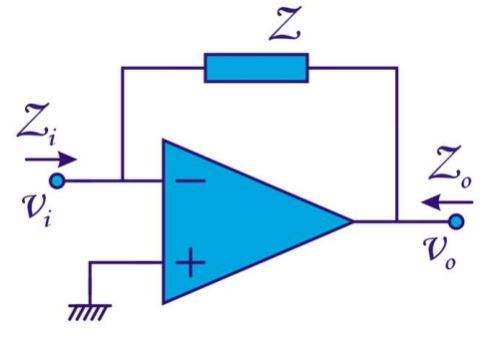
\includegraphics[width=7cm]{figures/ch10/feedback4.jpg}
	\captionof{figure}{}
	\label{fig:feedback4}
\end{minipage}%
\begin{minipage}{.5\textwidth}
	\centering
	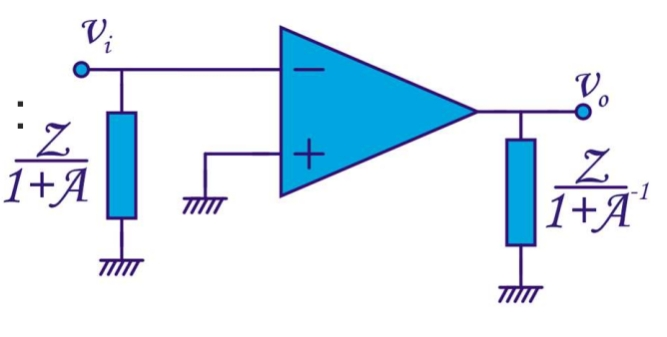
\includegraphics[width=7cm]{figures/ch10/feedback5.jpg}
	\captionof{figure}{}
	\label{fig:feedback5}
\end{minipage}

By using these relations, we can redraw the circuit as the one in figure \ref{fig:feedback5}, where we explicitly represented the in- and output impedances.

\section{Increased bandwidth}
Assume that the amplifier $A(j \omega)$ can be modeled as a system with a single pole in $\omega_0$:
$$
A(j \omega) = \frac{A_0}{1 + j \frac{\omega}{\omega_0}}
$$
Substituting this in the expression for the closed-loop gain $A_{CL}$ gives:
\begin{align*}
	A_{CL} &= \frac{A(j\omega)}{1 + A(j \omega) H} = \frac{\frac{A_0}{1 + j \frac{\omega}{\omega_0}}}{1 + \frac{A_0}{1 + j \frac{\omega}{\omega_0}} H} \\
			&= \frac{\omega_0 A_0}{(\omega_0 + j\omega) + \omega_0 A_0 H} = \frac{\omega_0 A_0}{(1 + T_0) \omega_0 + j\omega} \\
			&= \frac{\frac{A_0}{1 + T_0}}{1 + j \frac{\omega}{\omega_0 (1 + T_0)}}
\end{align*}
So the closed-loop system is also a first-order system, but now:
\begin{itemize}
	\item The gain $A_0$ is divided by the loop gain plus one.
	\item The bandwidth is increased by the same factor because the pole lies in $\omega_0 (1 + T_0)$.
	\item The gain-bandwidth product $GBW$ remains constant.
\end{itemize}
This is the same conclusion as in figure \ref{fig:opamp11}.

\section{Distortion reduction}
% video 17 45:00
We model a distortion as an unwanted signal somewhere downstream in out circuit. Take for example the circuit in figure \ref{fig:feedback6}, where the first amplifier is an OPAMP, and the second is a class B push-pull amplifier, like in figure \ref{fig:pushpull3}, including the feedback path through $R_1$ and $R_2$, modeled with $H(j\omega)$. The second amplifier suffers from a large distortion, modeled as a voltage $v_d$ applied at its input.
\begin{figure}[h!]
	\centering
	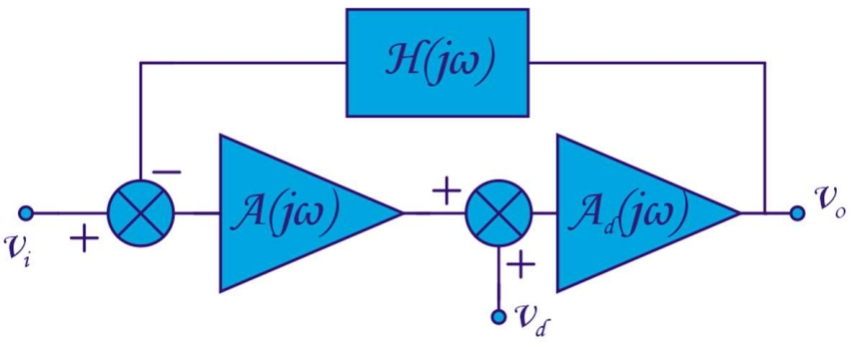
\includegraphics[width=12cm]{figures/ch10/feedback6.jpg}
	\caption{}
	\label{fig:feedback6}
\end{figure}
Without feedback, this distortion is directly visible at the output, magnified by the gain $A_d$ : $v_o = A(j\omega) A_d(j\omega) \; v_i + A_d(j\omega) v_d$. However, with feedback this becomes:
\begin{align*}
	v_o &= A_d(v_d + A(v_i - H v_o))\\
	(1 + A_dAH)\; v_o &= A_d v_d + A_d A v_i \\
	v_o &= \frac{AA_d}{1 + T} v_i + \frac{A_d}{1 + T} v_d \\
		&\approx \frac{1}{H} v_i + \frac{1}{AH} v_d
\end{align*} 
with the loop gain $T = A A_d H$. This means that the distortion is reduced by a factor $A$ compared to the input signal. Knowing that a distortion downstream will be reduced by the gain of the previous stages, it is important to place a distortion-less amplifier as the first stage of the loop.\\
In the circuit in figure \ref{fig:pushpull3}, we needed diodes as a pre-bias to avoid cross-distortion. But thanks to the feedback, if you would omit the diodes in the second stage of figure \ref{fig:feedback6}, there would be no distortion either, because every distortion in the second stage will be divided by $A$.


%\section{Feedback and OPAMP}

%\section{The Emitter Resistance  and Feedback}

\section{Stability Issues}

To keep the operating point of the OPAMP with feedback stable, it is essential that we apply the feedback to the negative terminal. Otherwise, the system becomes unstable and the output will go to infinity (will explode) - in reality, off course, the output will be set to the OPAMP supply $\pm E$.\\
In principle, we can analyze the frequency response of the feedback topology in figure \ref{fig:feedback_general} by expressing both the Laplace transforms on  $A(s)$ and $H(s)$ as the ratio of two polynomials\footnote{Note that $s=\sigma + j \omega$. We usually set $\sigma=0$, i.e. we analyze the frequency response of the system.}:
$$
A(s) = \frac{N_A(s)}{D_A(s)} \text{ and }
H(s) = \frac{N_H(s)}{D_H(s)}
$$
and substituting in the expression for the closed-loop \ref{eq:closed-loop}:
\begin{align*}
	A_{CL}(s) &= \frac{A(s)}{1 + A(s) H(s)} = \frac{\frac{N_A(s)}{D_A(s)}}{1 + \frac{N_A(s)}{D_A(s)} \frac{N_H(s)}{D_H(s)}} \\
			  &= \frac{N_A(s) D_H(s)}{ D_A(s) D_H(s) + N_A(s)N_H(s)}
\end{align*}
To verify the stability, we must calculate the poles and check wether their real part is negative (i.e. do they lie in the left half of the s-plane) - see section \ref{sec:laplace}. If this is the case for all poles, the system is asymptotically stable. However, to find the poles, we must solve $D_A(s) D_H(s) + N_A(s)N_H(s) = 0$. This method is usually very complex because it requires the factoring of high-order polynomials, and it gives no indication of the stability margins, i.e. how much can the different parameters vary before the system becomes unstable.\\
Let's take another approach. We will assume that the open loop gain $A(j\omega)$ is low-pass: i.e. it has a pole in $\omega = \omega_d$ and for all frequencies $\omega <\omega_d$, $A(j \omega) = A_0$ is constant. For all $\omega > \omega_d$ the gain decreases. This means we model $A(j\omega)$ with following expression, where $\omega_d$ is the dominant pole and $\omega_{nd}$ is the non-dominant pole \footnote{In general, there can be many of those non-dominating poles; what is important is that the $\omega_d$ determines the low-frequency behavior.}:
$$
A(j \omega) = \frac{A_0}{(1 + j\frac{\omega}{\omega_d})(1 + j\frac{\omega}{\omega_{nd}})}
$$
With $T(j\omega) = A(j\omega) H(j\omega)$, we know that the closed-loop gain is
$$
A_{CL} = \frac{A(j\omega)}{1 + T(j\omega)}
$$
This means that if $T(j\omega) > 0$ the system is always stable. The problem arises when $T(j \omega) = -1$, i.e. if for a certain $\omega_\phi$:
\begin{itemize}
	\item $|T(\omega_\phi) = 1$, and
	\item $\angle T(\omega_\phi)) = 180^\circ$
\end{itemize}
So even when we apply feedback to the negative terminal, if the frequency response is such that the signal undergoes an additional phase shift of $180$°, it can create an unstable circuit. The magnitude at the frequency $\omega$ where this phase shift happens must be $\ge 1$ for this unstable behavior to be sustained.\\
To demonstrate this, consider the topology in figure \ref{fig:feedback7}. We established earlier that $T = \frac{R_1}{R_1 + R_2} A(j\omega)$. Notice that the feedback is applied to the negative terminal. A small perturbation that occurs at the negative input, as shown by the up arrow, will be amplified and becomes a larger perturbation at the output, but in the other direction. This output perturbation will be transmitted to the input by the feedback path but, as long as $T > 0$, \textbf{will act against the original perturbation}. The perturbation can not be sustained and will die out. The circuit is unconditionally stable.\\
Now assume the feedback is done on the positive terminal as in figure \ref{fig:feedback8}. The perturbation will travel around the circuit and will arrive back with the same direction at the input node. This means that the perturbation will not only be sustained but magnified, and the system becomes unstable. Note that this situation would be identical to the one in figure \ref{fig:feedback7} if $T$ were negative.\\


\begin{minipage}{.5\textwidth}
	\centering
	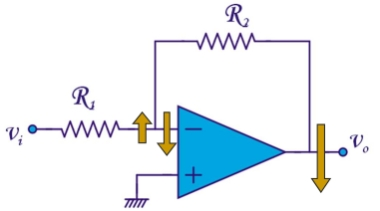
\includegraphics[width=7cm]{figures/ch10/feedback7.jpg}
	\captionof{figure}{}
	\label{fig:feedback7}
\end{minipage}%
\begin{minipage}{.5\textwidth}
	\centering
	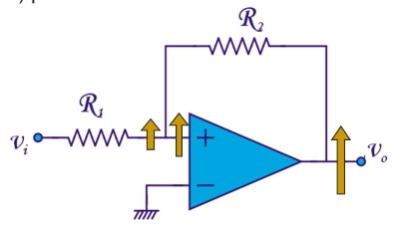
\includegraphics[width=7cm]{figures/ch10/feedback8.jpg}
	\captionof{figure}{}
	\label{fig:feedback8}
\end{minipage}

If $H$ has no frequency dependence and $A(j\omega)$ has a single pole $\omega_d$, we can solve the problem analytically. With $A(j\omega) = \frac{A_0}{1 + j\frac{\omega}{\omega_d}}$, we find for the (closed) loop gain:
$$
T(j\omega) = \frac{A_0 H}{1 + j\frac{\omega}{\omega_d}} \text{ and } A_{CL} = \frac{A_0}{1 + A_0H} \frac{1}{1 + j \frac{\omega}{\omega_d(1 + A_0 H)}} = \frac{A_{CL0}}{1 + j\frac{\omega}{\omega_{CL}}}
$$
which is a result we already found when we discussed the increased bandwidth. Interpreting this as the movement of pole in the $s$-plane, we see that the existing pole $\omega_d$ has moved to the left: 
$$\omega_{CL} = (1 + A_0H) \; \omega_d$$
This movement is shown in figure \ref{fig:feedback9}. This is the \emph{root-locus}, because it traces how the root(s) (poles) of the closed-loop response move as function of $H$. The closed-loop always remains stable. This can also been learned from the Bode curve, because a first-order system can only have a maximal phase shift of $90$°, and not $180$° as needed for an instability.

\begin{minipage}{.5\textwidth}
	\centering
	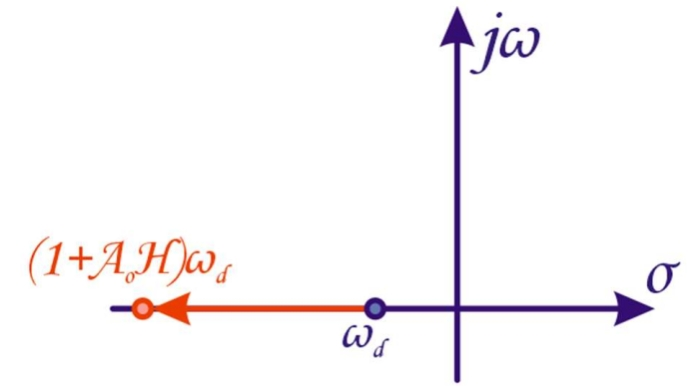
\includegraphics[width=7cm]{figures/ch10/feedback9.jpg}
	\captionof{figure}{}
	\label{fig:feedback9}
\end{minipage}%
\begin{minipage}{.5\textwidth}
	\centering
	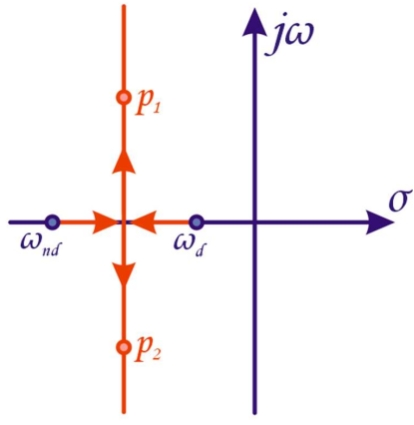
\includegraphics[width=5cm]{figures/ch10/feedback10.jpg}
	\captionof{figure}{}
	\label{fig:feedback10}
\end{minipage}

We can do the same analysis for a system with two poles, where $A(j\omega)$ is given by:
$$
A(j \omega) = \frac{A_0}{(1 + \frac{\omega}{\omega_d})(1 + \frac{\omega}{\omega_{nd}})}
$$
with $\omega_d$ the dominant and $\omega_{nd}$ the non-dominant pole, as before. Then:
$$T(j\omega) = A(j\omega) H(j\omega) = \frac{A_0 H}{(1 + \frac{\omega}{\omega_d})(1 + \frac{\omega}{\omega_{nd}})}$$
and
$$
A_{CL} = \frac{A(j\omega)}{1 + T(j\omega)} = \frac{A_0 \omega_d \omega_{nd}}{(1 + A_o H) \omega_d \omega_{nd} + j\omega(\omega_d + \omega_{nd}) - \omega^2}
$$
The poles of $A_{CL}$ are found by solving for the roots of the denominator. The result is:
\begin{align*}
p_{1, 2} &= -\frac{1}{2}(\omega_d + \omega_{nd}) \pm \frac{1}{2} \sqrt{ (\omega_d + \omega_{nd})^2 - 4(1 + A_0H)\omega_d \omega_{nd}} \\
%		 &\approx -\frac{1}{2}\omega_{nd} \pm \frac{1}{2} \sqrt{ \omega_{nd}^2 - 4\omega_{CL_d} \omega_{nd}}
\end{align*}
This means that if $1+A_0H$ is small, the poles are real and located close to $-\omega_d$ and $-\omega_{nd}$. As $A_0H$ increases, they move closer together. At some point (i.e. when the part under the square root is zero) they collide and are both equal to $-\frac{1}{2}(\omega_d + \omega_{nd})$. If  $A_0H$ increases further, the term under the square root becomes negative and the poles acquire an imaginary part, i.e. they become complex when 
$$A_0H > \frac{(\omega_d - \omega_{nd})^2}{4 \omega_d \; \omega_{nd}} \approx \frac{\omega_{nd}}{4\omega_d}$$
This situation is represented in the root-locus of figure \ref{fig:feedback10}. Note how even for a second-order system, the poles always remain in the left half-plane and so the system stays stable. The imaginary component of the poles is reflected in the fact that the circuit may oscillate temporarily and may appear unstable. \\
The maximal phase-shift of a second order system is $180$°, but this shift only occurs when $\omega \rightarrow \infty$ so in practice the system will remain stable. This however does not mean that there are no issues. Even stable systems can have a large overshoot (i.e. how far goes the step response beyond its final value) in the step response, as in figure \ref{fig:feedback11}. This figure shows the step response of a second order system. In general, the transfer function of a second order system can be written as:
\begin{align}
	H(j \omega) = \frac{\omega_0^2}{\omega_0^2 +2j\zeta \omega_0 \omega - \omega^2}
\end{align}
with $\omega_0$ the eigenfrequency and $\zeta$ the damping ratio. The damping ratio $\zeta$ is related to the ratio of the imaginary and real component of the complex pole: if the poles are both real, $\zeta > 1$ and there are no oscillations; if $\zeta = 0$, the poles are imaginary and the system is undamped: even a small perturbation is enough to generate a continuous oscillation. If $\zeta$ is small, the overshoot is high, but the response is fast. Ideally, $\zeta \approx 0.46$ to have a reasonable fast step response without too much overshoot, as can be seen in figure \ref{fig:feedback10}.\\

\begin{figure}[h!]
	\centering
	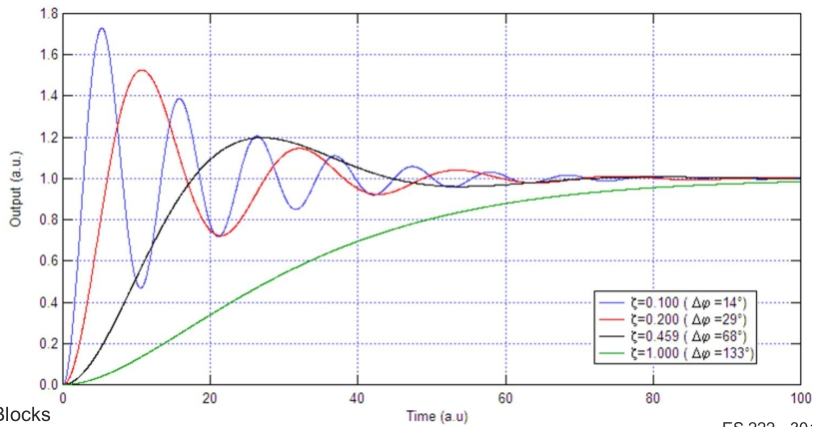
\includegraphics[width=14cm]{figures/ch10/feedback11.jpg}
	\caption{}
	\label{fig:feedback11}
\end{figure}
%$$\frac{\omega_0^2}{s^2 + 2\zeta \omega_0 s + \omega_0^2}$$
The damping ratio is related to the \emph{phase margin} $\Delta \phi$. This is the difference between the phase at the frequency where the gain is 0 dB (i.e. $A_v = 1$) and a phase of $180$°. Figure \ref{fig:feedback12} shows the (normalized) bode curves and phase margin for different values of $\zeta$. The ideal $\zeta$ corresponds to a phase margin $\Delta \phi = 68$°. If $\Delta \phi = 0$, the system is unstable. So in a sense the phase margin gives an indication how far we are from instability.

\begin{figure}[h!]
	\centering
	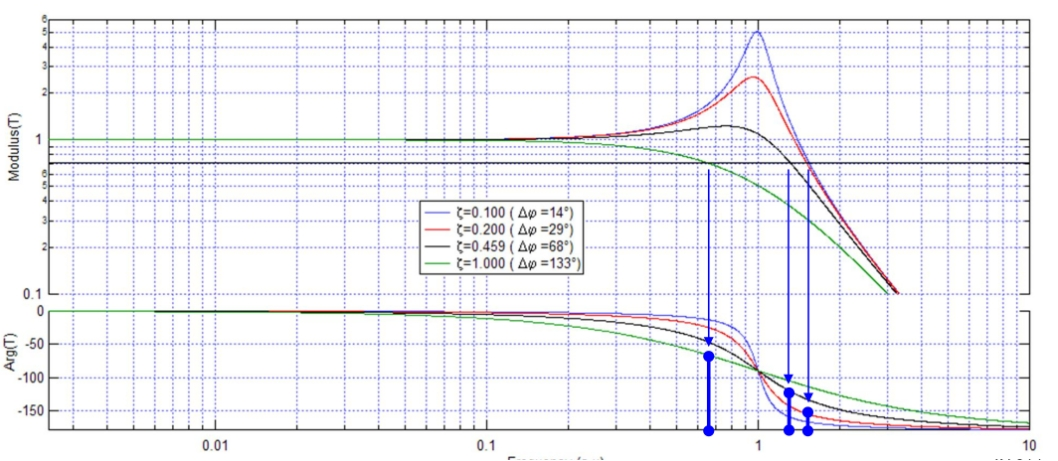
\includegraphics[width=14cm]{figures/ch10/feedback12.jpg}
	\caption{}
	\label{fig:feedback12}
\end{figure}

In summary we can say that (1) OPAMPs have multiple (2 or more) poles and (2) this will have an effect on circuit stability. This stability depends on the poles (and zeros) of the loop gain $T(j\omega)$ and thus implicitly on $A(j\omega)$ en $H(j\omega)$, of which the latter term is application dependent. In essence, there are two types of OPAMPS:
\begin{enumerate}
	\item Compensated OPAMPS: for these devices, as long as $|H(j\omega)| < 1$, stability is guaranteed. These circuits have a large phase margin, but are inherently slow because their bandwidth is artificially reduced.
	\item Uncompensated OPAMPS: no measures were taken to assure stability; the user is responsible for this. These devices do have maximal bandwidth.
\end{enumerate}